\documentclass{article}
\usepackage{graphicx}
\usepackage[utf8]{inputenc}
\usepackage{caption}

\setlength\fboxsep{0pt}
\setlength\fboxrule{0.5pt}

\title{
    System design document for group 16
    \author{Erik Sjöström,
            Filip Labe,
            Jonatan Källman,
            Sarosh J. Nasir}
    \date{\today \\v1.0}         
}

\begin{document}
\maketitle

\section{Introduction}

\subsection{Design Goals}

Monster Clicker is a mobile game for Android. So the program must therfore run on Android,
it must be able to get input from the user, and display the result of these inputs. 

\subsection{Definitions, acronyms, abbriviations}
\begin{itemize}
    \item \emph{Monster Clicker} - The name of the project.
\end{itemize}

\section{System architecture}

Monster Clicker starts when the user opens the application. From there the user has
the option of visiting several different activities. Each activity presents and
represents different use cases such as, buying upgrades, viewing the map, attacking monsters, etc. \\ \noindent
Monster Clicker ends when the user either exits the app or closes it using the android application manager.

\subsection{Programming patterns}
Monster Clicker, just like any other piece of software relies on different design/architecture patterns, such as:
\begin{itemize}
    \item Game Loop \cite{game-loop}
    \item Model View Presenter \cite{MVP}
    \item Singelton-pattern
    \item Factory-pattern
\end{itemize}

\subsection{Dependencies}
Monster Clicker is a self contained piece of software, whch means that it does not
depend on anything but itself. The application contains all the information 
required to be able to run. \\

\noindent
The application is subdivided into several packages:
\begin{itemize}
    \item \emph{Player:} this package contains a player model, and an interface for this model. The model contains the state of the player, damage, gold, etc. And methods to access and/or change the state.
    \item \emph{Monster Pack}
    \item \emph{Map}
    \item \emph{Stats}
    \item \emph{Upgrades}
    \item \emph{Clock}
\end{itemize}

\noindent
Gem Clicker is developed for the Android operating system and is guaranteed to
run on android phones running 4.0 or later versions of the operating system.  

\section{Subsystem decomposition}

\subsection{Player}
This package contains a player model, and an interface for this model. The model contains the state of the player, damage, gold, etc. And methods to access and/or change the state. The interface provides a layer between the model and anyone who wishes to access it, only exposing non-internal methods.
\newpage
\subsubsection{Diagrams}
\begin{center}
    Sequence diagram of getState()\\
    \fbox{ 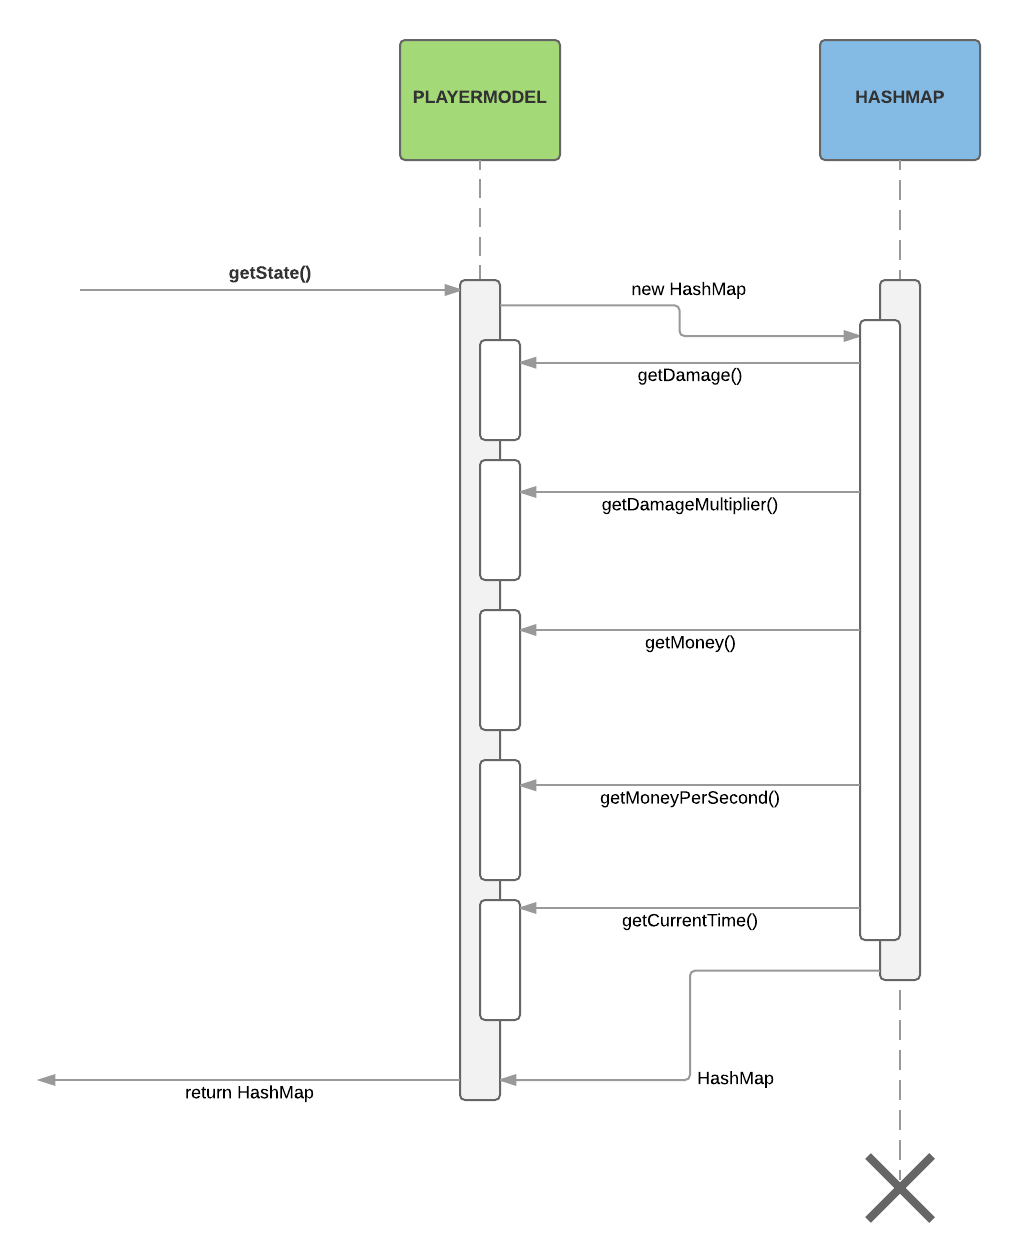
\includegraphics[scale=0.3]{seqDiagrams/playerModel.png}}
\end{center}

\subsubsection{Quality}
The tests for \emph{PlayerModel} can be found in \emph{/OOPP/app/src/test/\ldots/oopp/PlayerModelTest.java}

\subsection{Monster Pack}
This package contains a monster model, and a monster factory. The model contains the state of the monster, gold, health, etc. A constructor to set the state and methods
to modify the state. The factory handles the creation of monsters in a simplified way.

\subsection{Map}

\subsection{Stats}

\subsection{Upgrades}

\subsection{Clock}

\section{Persistent data management}
Gem Clicker saves the state of the app when the app is closed. 
This data is represented as a simple text file, and doesn't take up any noticible space on the users phone.

\section{Access control and security}
There are no different roles for using this application. The only role is that of the user,
and the only permission required of the user is to use the storage space of the phone.

\section{References}
\begin{thebibliography}{9}
    
    \bibitem{game-loop}
        http://gameprogrammingpatterns.com/game-loop.html
    
    \bibitem{MVP}
        https://en.wikipedia.org/wiki/Model–view–presenter

\end{thebibliography}

\end{document}
